\documentclass{standalone}

\usepackage{tikz}
\usepackage{pgfplots}
\usepackage[cmex10]{amsmath}
\usepackage{amsfonts}
 \pgfplotsset{compat=1.12}
%\usepgfplotslibrary{polar}

\begin{document}

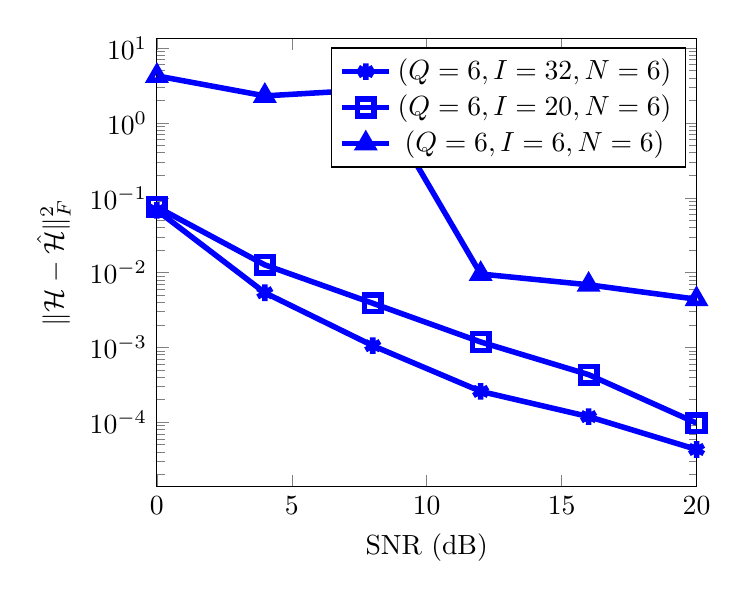
\begin{tikzpicture}

  \begin{axis}[%
    ymode = log,
%scale only axis,
%separate axis lines,
%every outer x axis line/.append style={black},
%every x tick label/.append style={font=\color{black}},
xmin=0,
xmax=20,
xlabel={SNR (dB)},
%xmajorgrids,
%every outer y axis line/.append style={black},
%every y tick label/.append style={font=\color{black}},
ylabel={ $\|\mathcal{H} - \hat{\mathcal{H}}\|^2_F$},
%title = Channel frequency response between $\mathbf{H}(2,1)$,
%ymajorgrids,
%axis background/.style={fill=white},
%legend style={at={(0.55,0.85)},anchor=south west,legend cell align=left,align=left,draw=black}
]

%%%%%%%%%%%%%%%%%%%%%%%%% M=8 %%%%%%%%%%%%%%%%%%%%%%%%%%%%%%%%%%%%%%%%%%%%%%%%%


\addplot [color=blue,solid,mark=asterisk,mark options={solid},line width=2pt,mark size=3pt]
  table[row sep=crcr]{%
0 0.068043 \\
4 0.0053826 \\
8 0.0010556 \\
12 0.00025863 \\
16 0.00011893 \\
20 4.3264e-05 \\   
};
\addlegendentry{$(Q=6,I=32,N=6)$}; 


\addplot [color=blue,solid,mark=square,mark options={solid},line width=2pt,mark size=3pt]
  table[row sep=crcr]{%
0 0.075305 \\
4 0.012687 \\
8 0.0038946 \\
12 0.0011827 \\
16 0.0004329 \\
20 9.7412e-05 \\   
};
\addlegendentry{$(Q=6,I=20,N=6)$};

\addplot [color=blue,solid,mark=triangle,mark options={solid},line width=2pt,mark size=3pt]
  table[row sep=crcr]{%
0 4.2616 \\
4 2.3019 \\
8 2.794 \\
12 0.0095793 \\
16 0.0068733 \\
20 0.004409 \\
};
\addlegendentry{$(Q=6,I=6,N=6)$};



\end{axis}
\end{tikzpicture}%
\end{document}

%%% Local Variables:
%%% mode: latex
%%% TeX-master: t
%%% End:
